\documentclass[a4paper,fleqn]{article}
\title{Rapport}
\author{P\aa b\o l}

\usepackage{fancyhdr}
\usepackage{amsmath}
\usepackage{amssymb}
\usepackage{tikz}
\usepackage{pgfplots}
\usepackage{graphicx}
\graphicspath{ {images/} }
\usepackage[danish]{babel}
\usepackage[utf8]{inputenc}
\usepackage{lastpage}
\usepackage{lipsum}
\usepackage[colorlinks, linkcolor=black]{hyperref}
\usepackage{listings}
\usepackage{upquote}

\definecolor{bluekeywords}{rgb}{0.13,0.13,1}
\definecolor{greencomments}{rgb}{0,0.5,0}
\definecolor{redstrings}{rgb}{0.9,0,0} 
\newcommand{\hmwkTitle}{Projekt C} % Assignment title
\newcommand{\hmwkDueDate}{31/05\ -\ 2019} % Due date
\newcommand{\hmwkClass}{Lineær algebra} % Course/class
\newcommand{\hmwkClassInstructor}{Lærer: $Henrik^2$} % Teacher/lecturer
\newcommand{\hmwkAuthorName}{Christian P\aa b\o l} % Your name
\newcommand{\hmwkProblem}{}

% Big fugly math letters
\newcommand{\RR}{\mathbb{R}}
\newcommand{\U}{\mathcal{U}}
\newcommand{\A}{\mathcal{A}}
\newcommand{\B}{\mathcal{B}}
\newcommand{\Q}{\mathcal{Q}}

\addtolength{\oddsidemargin}{-.875in}
\addtolength{\evensidemargin}{-.875in}
\addtolength{\textwidth}{1.75in}
\setlength{\parindent}{0in}

\pagestyle{fancy}
\lhead{\hmwkAuthorName} % Top left header
\chead{\hmwkClass\ : \hmwkTitle} % Top center head
\rhead{\rightmark}
\cfoot{} % Bottom center footer
\rfoot{Page\ \thepage\ of\ \protect\pageref{LastPage}} % Bottom right footer

\date{} 

\title{
	\vspace{2in}
	\textmd{\textbf{\hmwkClass:\ \hmwkTitle}}\\
	\normalsize\vspace{0.1in}\small{Afleveres:\ \hmwkDueDate}\\
	\vspace{0.1in}\large{\textit{\hmwkClassInstructor}}\\
	\normalsize\vspace{0.5in} \hmwkProblem 
	\vspace{3in}
}

\author{\textbf{\hmwkAuthorName}}

\begin{document}
	\maketitle
	\newpage
	\setcounter{page}{1}
%  ___                                _ 
% / _ \ _ __   __ _  __ ___   _____  / |
%| | | | '_ \ / _` |/ _` \ \ / / _ \ | |
%| |_| | |_) | (_| | (_| |\ V /  __/ | |
% \___/| .__/ \__, |\__,_| \_/ \___| |_|
%      |_|    |___/                     
	\section{Opgave 1}
	Vi betragter underrummet $\U = span\{u_1,u_2\}$ af $\RR^3$ hvor
	\[ u_1 = \begin{pmatrix}3\\2\\6\end{pmatrix} \text{ og } 
	u_2=\begin{pmatrix}9\\-1\\4\end{pmatrix}\]
	
	\subsection{a}
	Bestem projektionsmatricen P for underrummet $\U$. Vi checker først at $u_1,u_2$ er en
	basis, ved at observere $Rank [u_1|u_2] = 2$ og at der derfor ingen frie variabler er.
	Så checker vi om de er ortogonale på hinanden $u_1 \perp u_2$?
	\[ u_1 \bullet u_2 = 49 \neq 0 \]
	Så vi skal finde en ortogonal eller ortonormal basis for underrummet $\U$. Her kan vi
	bruge Gram-Schmidt processen til at finde en. Vi finder frem til $q_1,q_2$ som er
	ortogonale på hinanden, og skalerer dem så med deres længde for at få vektorer af længde
	1 og dermed en ortonormal basis.\\
	Vi opstiller $q_1$ som $u_1$ og normaliserer:
	\[ q_1 = \frac{u_1}{||u_1||} = \frac{1}{7}\begin{pmatrix}3\\2\\6\end{pmatrix} \]
	Vi projekterer $u_2$ i $q_1$ og trækker det fra $u_2$
	\[ q'_2 = u_2 - (u_2\bullet q_1)q_1 = u_2 - 7 \cdot (\frac{1}{7}u_1) = u_2 - u_1 =
	\begin{pmatrix}6\\-3\\-2\end{pmatrix}\]
	Vi Normaliserer så $q'_2$ 
	\[ q_2 = \frac{q'_2}{||q'_2||} = \frac{1}{7}\begin{pmatrix}6\\-3\\-2\end{pmatrix}\]
	Vi har så et sæt $\{q_1,q_2\}$ som en ortonormal basis for underrummet $\U$.\\
	Formlen for projektionsmatricen for ortonormale baser er $QQ^T$. hvor $Q = [q_1|q_2]$. Vi
	opstiller derfor
	\[ P_\U = 
		\frac{1}{7}\left(\begin{array}{rr}
			3 & 6\\
			2 & -3\\
			6 & -2
		\end{array}\right)
		\cdot
		\frac{1}{7}\left(\begin{array}{rrr}
			3 & 2 & 6\\
			6 & -3 & -2
		\end{array}\right)
		= 
		\frac{1}{49}\begin{pmatrix}
			45&-12&6\\
			-12&13&18\\
			6&18&40
		\end{pmatrix}
	\]

	\subsection{b}
	Bestem spejlingen af vektoren $e_1 = \begin{pmatrix}1\\0\\0\end{pmatrix}$ i underrummet
	$\U$\\
	For at finde spejlingen af $e_1$ i $\U$ kan vi udregne $2Pe_1 - e_1$
	\[ 2P \begin{pmatrix}1\\0\\0\end{pmatrix} = 
	\frac{1}{49}\begin{pmatrix}90\\-24\\12\end{pmatrix} - e_1
	 = \frac{1}{49}\begin{pmatrix}41\\-24\\12\end{pmatrix}
	\]

	\subsection{c}
	Bestem en basis ${u_3}$ for underrummet $\U^\perp$. \\
	Da $\dim \U = 2$ må $\dim \U^\perp = 1$. Vi skal derfor finde en vektor $v$ hvor produktet
	af $u_1 \cdot v = 0$ og $u_2 \cdot v = 0$. Dette kan skrives $\U^Tv = 0$. Vi opstiller
	en totalmatrice og sætter på reduceret rækkeechelonform
	\begin{equation*}
		\left(\begin{array}{rrr|r}
			3 & 2 & 6 & 0 \\
			9 & -1 & 4 & 0
		\end{array}\right)
		\begin{array}{l}
			\frac{1}{3}r_1 \rightarrow r_1\\
			r_2 - 9r_1 \rightarrow r_2\\
			-\frac{1}{7}r_2 \rightarrow r_2\\
			r_1 - \frac{2}{3}r_2 \rightarrow r_1\\
		\end{array} \rightsquigarrow
		\left(\begin{array}{rrrr}
			1 & 0 & \frac{2}{3} & 0 \\
			0 & 1 & 2 & 0
		\end{array}\right)
	\end{equation*}
	Vi opstiller løsningsmængden:
	\[ v = t\begin{pmatrix}
			-\frac{2}{3}\\
			-2\\
			1\\
		\end{pmatrix}
	\]
	Og 
	\[ \U^\perp = \text{span} \left\{\begin{array}{c}-\frac{2}{3}\\-2\\1\\\end{array}\right\}\]


	\subsection{d}
	Bestem forskriften for den lineære transformaion $T: \RR^3 \rightarrow \RR^3$ som opfylder:
	\[ T(u_1) = u_2 \quad T(u_2) = u_1 \quad T(u_3) = u_3 \]
	Vi ser her at $T$s formål er at bytte om på $u_1 \rightarrow u_2$. Dette kan også opstilles
	som en rækkeoperation. Vi opstiller derfor en matrice:
	\[ P = \begin{bmatrix}0&1&0\\1&0&0\\0&0&1\end{bmatrix} \]
	Som er den tilsvarende elementærmatrice for rækkeoperationen $r_1 \leftrightarrow r_2$.
	Vi kigger så på $PU^T$.\footnote{Hvor U er transponeret, da vi skal have vektorer i rækker,
	og ikke søjler, så de ganges sammen ind i matricen $u_{11} \cdot P_{11}$ etc.}
	\[ \begin{bmatrix}0&1&0\\1&0&0\\0&0&1\end{bmatrix}
	\begin{pmatrix}3&2&6\\9&-1&4\\-\frac{2}{3}&-2&1\end{pmatrix}
	= 
	\begin{pmatrix}9&-1&4\\3&2&6\\-\frac{2}{3}&-2&1\end{pmatrix}
	\] Vi ser her at $P$ korrekt laver $u_1 \leftrightarrow u_2$ og lader $u_3$ stå uberørt,
	og vi siger derfor $P$ er forskriften for $T$.\\

	Det nævnes at dette ikke er en generel løsning for at finde forskriften. Blot en genvej.


%  ___                                ____  
% / _ \ _ __   __ _  __ ___   _____  |___ \ 
%| | | | '_ \ / _` |/ _` \ \ / / _ \   __) |
%| |_| | |_) | (_| | (_| |\ V /  __/  / __/ 
% \___/| .__/ \__, |\__,_| \_/ \___| |_____|
%      |_|    |___/                         
	\section{Opgave 2}
	Vi betragter matricen
	\[A = \begin{pmatrix}
			1 & -3 & 8 & -1\\
			-4 & -3 & -2 & -2\\
			2 & 4 & 1 & 3\\
			2 & 4 & 16 & 1\\
	\end{pmatrix}\]

	\subsection{a}
	Bestem en QR-faktorisering af $A$\\
	For at regne en QR faktorisering af $A$ skal vi opstille to matricer $Q,R$ således at
	$QR = A$ hvor $Q = (q_1|\dots|q_j)$ fra Gram-Schmidt processen og $r_{ij} = q_i \bullet
	u_j$ for $i < j$ og $r_{jj} = ||u_j - r_{1j}q_1 - r_{2j}q_2-\cdots-r_{j-1,j}q_{j-1}||$\\
	Vi udfører nu Gram-Schmidt processen på A, hvor $u$ er søjlevektorer i $A$. Vi siger
	\begin{equation}
		\begin{array}{ll}
r_{11} = ||u_1|| = 5 & q_1 = \frac{u_1}{r_{11}} = \frac{1}{5} \begin{pmatrix} 5\\-4\\2\\2\end{pmatrix}\\
r_{12} = q_1 \bullet u_2 = 5 & q`_2 = u_2 - r_{12}q_1 = \begin{pmatrix}-4\\1\\2\\2\end{pmatrix}\\
r_{22} = ||q'_2|| = 5 & q_2 = \frac{1}{5}\begin{pmatrix}-4\\1\\2\\2\end{pmatrix}\\
r_{13} = q_1 \bullet u_3 = 10 & \\
r_{23} = q_2 \bullet u_3 = 0 & q'_3 = u_3 - r_{13}q_1 - r_{23}q_2 = \begin{pmatrix}6\\6\\-3\\12\end{pmatrix}\\
r_{33} = ||q'_3|| = 15 & q_3 = \frac{q'_3}{r_{33}} = \begin{pmatrix}2/5\\2/5\\-1/5\\4/5\end{pmatrix}\\
r_{14} = q_1 \bullet u_4 = 3 & \\
r_{24} = q_2 \bullet u_4 = 2 & \\
r_{34} = q_3 \bullet u_4 = -1& q'_4 = u_4 - r_{14}q_1 - r_{24}q_2 - r_{34}q_3 = \begin{pmatrix}2/5\\2/5\\4/5\\-1/5\end{pmatrix}\\
r_{44} = ||q'_4|| = 1 & q_4 = \frac{1}{1}q'_4 = \begin{pmatrix}2/5\\2/5\\4/5\\-1/5\end{pmatrix}
		\end{array}
	\end{equation}

	Vi har derfor matricerne $Q,R$ = 
	\[ Q = \left(\begin{array}{rrrr}
0.2 & -0.8 & 0.4 & 0.4 \\
-0.8 & 0.2 & 0.4 & 0.4 \\
0.4 & 0.4 & -0.2 & 0.8 \\
0.4 & 0.4 & 0.8 & -0.2
\end{array}\right),\qquad 
	R =\left(\begin{array}{rrrr}
5 & 5 & 10 & 3 \\
0 & 5 & 0 & 2 \\
0 & 0 & 15 & -1 \\
0 & 0 & 0 & 1
\end{array}\right)
\] Vi efterchecker dette svar ved at checke $QR = A$\\


	Vi betragter den vilkårlige matrice 
	\[ R = \begin{pmatrix}
			r_{11} & r_{12} & r_{13} & r_{14}\\
			0 & r_{22} & r_{23} & r_{24}\\
			0 & 0 & r_{33} & r_{34}\\
			0 & 0 & 0 & r_{44} \\
	\end{pmatrix}\]
	Hvor produktet $d = r_{11}r_{22}r_{33}r_{44}$ er forskelligt fra nul. Vi har så fået at
	vide at den inverse til den matrice er:
	\[R^{-1} = \frac{1}{d} \begin{pmatrix}
			r_{22}r_{33}r_{44} & -r_{12}r_{33}r_{44} & (r_{12}r_{23} - r_{13}r_{22})r_{44} & -r_{12}(r_{23}r_{34} - r_{24}r_{33} ) + r_{22}(r_{13}r_{34} - r_{14}r_{33})\\
			0& r_{11}r_{33}r_{44} &-r_{11} r_{23} r_{44} & r_{11}(r_{23}r_{34} - r_{24}r_{33})\\
			0&0&r_{11}r_{22}r_{44}&-r_{11}r_{22}r_{34}\\
			0&0&0&r_{11}r_{22}r_{33}
	\end{pmatrix}\]	

	\subsection{b}
	Benyt del (a) og ovenstående formel for $R^{-1}$ til at beregne $A^{-1}$\\
	Da vi har $A = QR$ kan vi opstille $A^{-1} = R^{-1}Q^{-1}$. Vi udnyter så at $Q$ er en 
	ortogonal matrice og $Q^{-1} = Q^T$, og opstiller derfor $A^{-1}Q^T$. Vi har formlen for
	$R^{-1}$ givet ovenfor, så vi skriver
	\[ d = r_{11}r_{22}r_{33}r_{44} = 375 \]
	\[
		R^{-1} = \begin{pmatrix}
			0.2 & -0.2 & -2/15 & -1/3\\
			0 & 0.2 & 0 & -0.4\\
			0 & 0 & 1/15 & 1/15\\
			0 & 0 & 0 & 1
		\end{pmatrix}
	\]
	Så opstiller vi 
	\[
		\begin{pmatrix}
			0.2 & -0.2 & -2/15 & -1/3\\
			0 & 0.2 & 0 & -0.4\\
			0 & 0 & 1/15 & 1/15\\
			0 & 0 & 0 & 1
		\end{pmatrix}
		\left(\begin{array}{rrrr}
			0.2 & -0.8 & 0.4 & 0.4 \\
			-0.8 & 0.2 & 0.4 & 0.4 \\
			0.4 & 0.4 & -0.2 & 0.8 \\
			0.4 & 0.4 & 0.8 & -0.2
		\end{array}\right) = 
		\left(\begin{array}{rrrr}
		\frac{1}{75} & -\frac{29}{75} & -0.24 & -0.04 \\
		-0.32 & -0.12 & -0.24 & 0.16 \\
		\frac{4}{75} & \frac{4}{75} & 0.04 & 0.04 \\
		0.4 & 0.4 & 0.8 & -0.2
		\end{array}\right) = A^{-1}
	\]
	\\
		
	\subsection{c}
	Vi ser $A = (a_1|a_2|a_3|a_4)$ og $Q = (q_1|q_2|q_3|q_4)$ hvor Q er den matrix fundet i
	QR faktorisering i (a). Vi betragter baserne $\A = \{ a_1, a_2, a_3, a_4 \}$ og $\Q
	= \{q_1, q_2, q_3, q_4 \}$ for $\RR^4$\\
	Vi viser nu at $P_{Q\leftarrow A} = R$\\

	Da $\A$ og $\Q$ udspænder samme rum, vil vi kunne udtrykke enhver vektor $x$ som
	koordinater i både $\A$ og $\Q$. Vi skriver det $[x]_\A = \A x, [x]_\Q = Qx$ for x udtrykt
	ved hhv. $\A$ og $\Q$. Da vi så har $\A = QR$ kan vi skrive $\A x = QRx$. Vi ser nu at $Rx$
	giver en ny vektor, som vi kalder $x'$ og opskriver $\A x = Qx'$. Vi ser vi nu har to sæt
	koordinater udtrykt ved A og Q, og at du kan gå fra $x$ til $x'$ ved at sige $x' = Rx$.
	Derfor vil en vektor udtrykt ved $\Q$ være $R\cdot [x]_\A = [x]_\Q$

	\subsection{d}
	Vi bestemmer nu tallene $\lambda_1 \lambda_2 \lambda_3 \lambda_4$ så vi har 
	$\lambda_1 a_1 + \lambda_2a_2 + \lambda_3a_3 + \lambda_4a_4 = 
	q_1 + q_2 +q_3 - \lambda_4q_4$\\
	Da begge sider af lighedstegnet er lineære kombinationer af A og Q. kan vi opskrive de to
	som koordinater:
	\[ [x]_\A = \begin{pmatrix}\lambda_1\\ \lambda_2\\\lambda_3\\\lambda_4\end{pmatrix}, \qquad
	   [x]_\Q = \begin{pmatrix}1\\1\\1\\-\lambda_4\end{pmatrix}
	\]
	Vi har så fra sidste opgave at $R[x]_\A = [x]_\Q$. Vi genkender her formen $Ax = b$ fra et
	lineært system, og opstiller $[R|[x]_\Q]$
	\[
		\left[\begin{array}{cccc|c}
			5 & 5 & 10 & 3 & 1\\
			0 & 5 & 0 & 2 & 1\\
			0 & 0 & 15 & -1 & 1\\
			0 & 0 & 0 & 1 & -\lambda_4\\
		\end{array}\right]
		\begin{array}{l}
			r_3 + 1r_4 \rightarrow r_3\\
			r_2 - 2r_4 \rightarrow r_2\\
			r_1 - 3r_4 \rightarrow r_1\\
			\frac{1}{15}r_3 \rightarrow r_3\\
			\frac{1}{5}r_2 \rightarrow r_2\\
			\frac{1}{5}r_1 \rightarrow r_1\\
			r_1 - 2r_3 \rightarrow r_1\\
			r_1 - 1r_2 \rightarrow r_1\\
		\end{array} \rightsquigarrow
		\left(\begin{array}{rrrr|r}
			1 & 0 & 0 & 0 & -\frac{1}{3} \, \lambda_4 - \frac{2}{15} \\
			0 & 1 & 0 & 0 & -\frac{2}{5} \, \lambda_4 + \frac{1}{5} \\
			0 & 0 & 1 & 0 & \frac{1}{15} \, \lambda_4 + \frac{1}{15} \\
			0 & 0 & 0 & 1 & \lambda_4
		\end{array}\right)
	\]
	Og vi opstiller derfor løsningsmængden
	\[\begin{pmatrix}\lambda_1\\\lambda_2\\\lambda_3\\\lambda_4\end{pmatrix} =
		\begin{pmatrix}
			-\frac{1}{3} \, \lambda_4 - \frac{2}{15} \\
			-\frac{2}{5} \, \lambda_4 + \frac{1}{5} \\
			\frac{1}{15} \, \lambda_4 + \frac{1}{15} \\
			\lambda_4
		\end{pmatrix}
	\]

%  ___                                _____ 
% / _ \ _ __   __ _  __ ___   _____  |___ / 
%| | | | '_ \ / _` |/ _` \ \ / / _ \   |_ \ 
%| |_| | |_) | (_| | (_| |\ V /  __/  ___) |
% \___/| .__/ \__, |\__,_| \_/ \___| |____/ 
%      |_|    |___/                         
	\section{Opgave 3}
	En computers regnekraft kan måles i flops, FLoating-point Operations Per Second. Vi vil
	benytte lineær algebra til at beskrive hvordan supercomputeres regnekraft har udviklet sig
	med tiden. Vi opskriver følgende historisk data for superkomputere. Derefter opskriver vi
	en tabel med flops(y) over tid, samt $\ln y$. \\
	\begin{tabular}{|c|c|c|}\hline
		År & Supercomputer & FLOPS\\\hline\hline
		2008 & IBM Roadrunner & $1.026\cdot 10^{15}$ \\
		2009 & Cray Jaguar & $1.759\cdot 10^{15}$ \\
		2010 & Tianhe-IA & $2.566\cdot 10^{15}$ \\
		2011 & Fujitsu K computer & $10.51\cdot 10^{15}$ \\
		2012 & IBM Sequoia & $16.32\cdot 10^{15}$ \\
		2013 & NUDT Tianhe-2 & $33.86\cdot 10^{15}$ \\
		2016 & Sunway TaihuLight & $93.00\cdot 10^{15}$ \\
		2018 & IBM Summit & $122.3\cdot 10^{15}$ \\\hline
	\end{tabular}\hspace{5em}
	\begin{tabular}{|c|c|c|}\hline
		t & y & ln y\\\hline\hline
		2008 & $1.026\cdot 10^{15}$ & $34.564$\\
		2009 & $1.759\cdot 10^{15}$ & $35.104$\\
		2010 & $2.566\cdot 10^{15}$ & $35.481$\\
		2011 & $10.51\cdot 10^{15}$ & $36.891$\\
		2012 & $16.32\cdot 10^{15}$ & $37.331$\\
		2013 & $33.86\cdot 10^{15}$ & $38.061$\\
		2016 & $93.00\cdot 10^{15}$ & $39.071$\\
		2018 & $122.3\cdot 10^{15}$ & $39.345$\\\hline
	\end{tabular}\\
	Det giver os data der ligner en eksponentiel kurve på y-aksen og punkter der næsten ligger
	på linje på $\ln y$ aksen. \\

	\subsection{a}
	Vi vil nu benytter mindste kvadraters metode, til at bestemme forskriften for den bedste
	rette linie, $\ln y \approx at+b$ gennem punkterne $(t, \ln y)$.\\
	Hvad vi vil gøre er at finde konstanter $a,b$ og derved en funktion: $at+b=\ln y$ og
	opstiller et ligningssystem $Ax = y$\\
	Da der ikke findes en ret linie gennem alle punkter $(t, \ln y)$ derfor er liningssystemet
	$Ax = b$ ikke konsistent. Vi vil derfor finde en vektor $\bar{x}$ der gør størrelsen
	$||A\bar{x} = b||$ mindst muligt. Processen der nu benyttes til at finde ligningen kaldes
	"mindste kvadraters metode" eller lineær regression.\\
	Før vi går helt igang, vil vi gøre det nemmere for os selv ved at bytte $t$ ud med $t'$
	hvor $t' = t-2008$. Dette giver os nogle lidt mindre tal længere nede, og gør det derfor
	mere overskueligt. Formlen vi regner er nu $a(t-2008) + b = \bar{y}$\\
	Vi har fra undervisningen at der findes følgende formel for at finde $\bar{x}$:
	\[ (A^T A)^{-1} A^T b = \bar{x} \]
	Vi skriver først $A$ og $A^T$ op.
	\[A = \left(\begin{array}{rr}
		0 & 1 \\
		1 & 1 \\
		2 & 1 \\
		3 & 1 \\
		4 & 1 \\
		5 & 1 \\
		8 & 1 \\
		10 & 1
	\end{array}\right), 
	A^T =\left(\begin{array}{rrrrrrrr}
		1 & 2 & 3 & 4 & 5 & 6 & 8 & 10 \\
		1 & 1 & 1 & 1 & 1 & 1 & 1 & 1
	\end{array}\right), b = \left(\begin{array}{r}
		34.564 \\
		35.104 \\
		35.481 \\
		36.891 \\
		37.331 \\
		38.061 \\
		39.071 \\
		39.345
	\end{array}\right) \]
	Vi bruger en matrixudregner til at regne produktet $(A^TA)$
	\[ (A^TA) = \left(\begin{array}{rr}
		219 & 33 \\
		33 & 8
	\end{array}\right)\]
	Og tager det inverse af det ved at bruge \verb!COMPUTATION! fra side 78 i bogen. Vi sætter
	$[(A^TA)|I_2] \rightsquigarrow [I_n|(A^TA)^{-1}]$ og får:
	\[ \left(\begin{array}{rr}
\frac{8}{663} & -\frac{11}{221} \\
-\frac{11}{221} & \frac{73}{221}
	\end{array}\right)\]
	Vi er nu ude i nogle wicked brøker, og sætter derfor pris på vore datalogiske
	forgængere der har lavet de værktøjer. Efter en kort bøn til vor frelser Dr. Richard
	Stallman, udregner vi nu $(A^TA)^{-1}A^T$
	\[\left(\begin{array}{rrrrrrrr}
		-\frac{11}{221} & -\frac{25}{663} & -\frac{1}{39} & -\frac{3}{221} & -\frac{1}{663} & \frac{7}{663} & \frac{31}{663} & \frac{47}{663} \\
		\frac{73}{221} & \frac{62}{221} & \frac{3}{13} & \frac{40}{221} & \frac{29}{221} & \frac{18}{221} & -\frac{15}{221} & -\frac{37}{221}
	\end{array}\right)\]
	Vi tørrer svedet af pandebåndet og priser os lykkelig over næsten at være færdig. Med 
	nyfunden respekt for matematikere før computere, opstiller vi $(A^TA)^{-1}A^Tb$
	\[\left(\begin{array}{r}
		0.506944193061840 \\
		34.8898552036199
\end{array}\right) = \bar{x} = \begin{pmatrix}a\\b\end{pmatrix}\approx \begin{pmatrix}0.507\\34.889\end{pmatrix}\]
	
Vi opstiller derfor funktionen $\bar{y} = 0.507(t-2008) + 34.889$. Set afbilledet på Figur~\ref{fig:weirdplot}
	\begin{figure}[!htb]
		\centering
		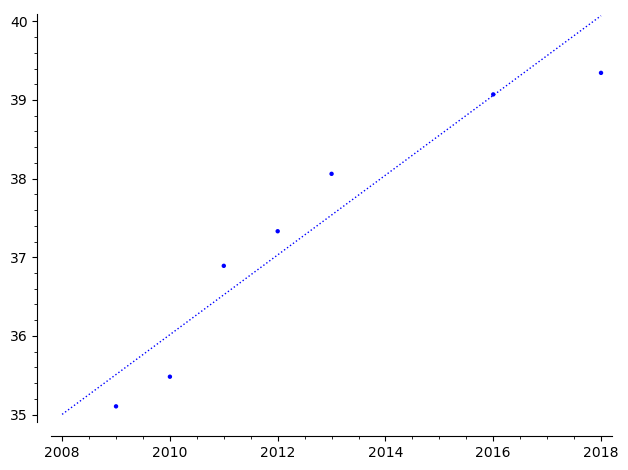
\includegraphics[width=0.4\linewidth]{3a.png}
		\caption{Plottet $\bar{y} = 0.507t' - 34.889$ samt de virkelige værdier}
		\label{fig:weirdplot}
	\end{figure}

	\subsection{b}
	Vi skal nu begrunde at følgende forskrift tilnærmelsesvist gælder for $y = y(t)$:
	\[ y = y(t) \approx 1.42\cdot 10^{15} \cdot e^{0.507(t-2008)}\]
	Hvad vi fandt tidligere var en funktion der udregnede $\ln y$. Vi kan så sige
	\[ \ln y = 0.507(t-2008) + 34.889 \leftrightarrow y = e^{0.507(t-2008) + 34.889}\]
	Og grundet potensreglen $a^{a+b} = a^{a} \cdot a^{b}$ siger vi
	\[ y = e^{34.889} \cdot e^{0.507(t-2008)} = 1.42\cdot10^{15} \cdot e^{0.507(t-2008)}\]
	Og vi ser så hvordan vi kommer frem til tilnærmelsen.

	\subsection{c}
	Vi bruger nu tilnærmelsen fra (b) til at regne hvor mange flops verdens bedste computer
	kunne udregne i 2000 og vil kunne i 2025. Hvis da vores udregning holder stik.
	\[ y(2000) = 2.459\cdot 10^{13}\]
	\[ y(2025) = 7.861\cdot10^{18}\]
	Da det faktiske tal for FLOPS dengang var $7.226\cdot 10^{12}$ ser vi at vores formel har
	en hvis mængde upræcision.
\end{document}
